\subsection{Computational graphs}

Another important concept is the one of \emph{computational graphs}.
A \emph{computational graph} describes a mathematical expression.
Such a \emph{directed graph} consists out of nodes and edges.
A node represents an arbitrary variable, that may be a scalar, a vector, a matrix or of any other type.
Then there are also \emph{operations}.
An \emph{operation} can be informally described as a label on a node.
This label defines the operation that is performed on the input.
Whereas the input is given by the \emph{directed edges} to that node.
An operation can take an arbitrary amount of inputs and stores the result in its node.

An example is given by \fref{fig:comp-graph-example}.

\begin{figure}[h]
    \centering
    \label{fig:comp-graph-example}
    
    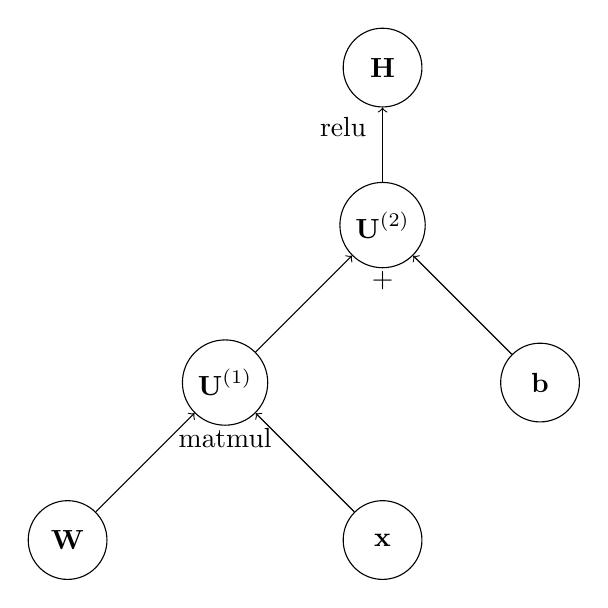
\begin{tikzpicture}
        \def\vert{2}
        \def\hori{2}
        \tikzstyle{place}=[circle, draw=black, minimum size=10mm]
        
        % Nodes
        \node[place] (w) at (0 * \hori, 0 * \vert) {\textbf{W}};
        \node[place] (x) at (2 * \hori, 0 * \vert) {\textbf{x}};
        
        \node[place, label={[shift={(0.0,-1.5)}]{\text{matmul}}}] (u1) at (1 * \hori, 1 * \vert) {$\textbf{U}^{(1)}$};
        \node[place] (b) at (3 * \hori, 1 * \vert) {\textbf{b}};
        
        
        \node[place, label={[shift={(0.0,-1.5)}]{\text{+}}}] (u2) at (2 * \hori, 2 * \vert) {$\textbf{U}^{(2)}$};
        
        \node[place, label={[shift={(-0.5,-1.5)}]{\text{relu}}}] (h) at (2 * \hori, 3 * \vert) {\textbf{H}};
        
        % Edges
        \draw [->] (w) to (u1);
        \draw [->] (x) to (u1);

        \draw [->] (u1) to (u2);
        \draw [->] (b) to (u2);
        
        \draw [->] (u2) to (h);
        
    \end{tikzpicture}
    \caption{Example of a computational graph}
\end{figure}